\chapter{Results}\label{chap:Results}

% Update?
% In this chapter, the results of the analysis are presented. \textbf{Chapter \ref{sec:Exploratory_Data_Analysis}} provides an overview of the data and explores the fairness of the dataset. 
% \textbf{Chapter \ref{sec:Results}} presents the results of the analysis. \textbf{Chapter \ref{sec:Limitations}} discusses the limitations of the analysis.

\section{Exploratory Data Analysis}\label{sec:Exploratory_Data_Analysis}



\subsection{Data Overview}\label{subsec:Data_Overview}

The processed dataset contained two \textit{numerical} features: \textbf{interest\_rate} and \textbf{loan\_to\_value\_ratio}.
Their distributions can be seen in \textbf{Figure \ref{fig:CHXX_Numerical_Distributions_1}} and \textbf{Figure \ref{fig:CHXX_Numerical_Distributions_2}}.

\begin{figure}[h]
    \centering
    \caption{Boxplots of the Numerical Features}
    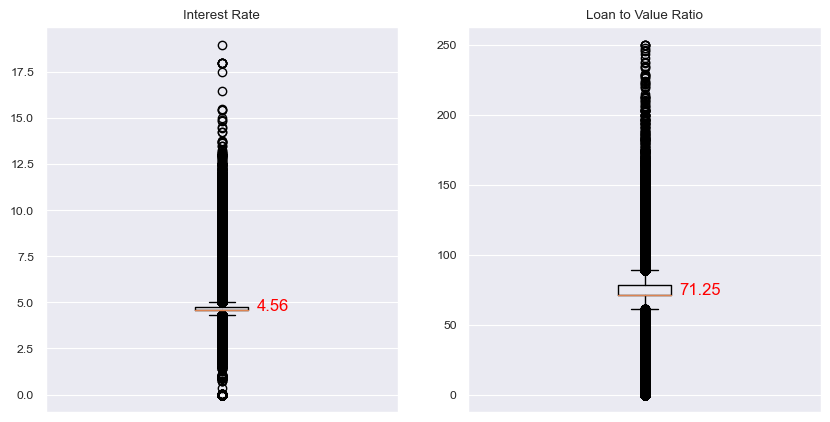
\includegraphics[width=0.85\textwidth]{CHXX_Numerical_Distributions_1.png}
    \caption*{The results of the KNNImputer applying mean (annotated in red) values for all missing values show clearly here by the narrow quartiles.}
    \label{fig:CHXX_Numerical_Distributions_1}
\end{figure}

\begin{figure}[h]
    \centering
    \caption{Histograms of the Numerical Features}
    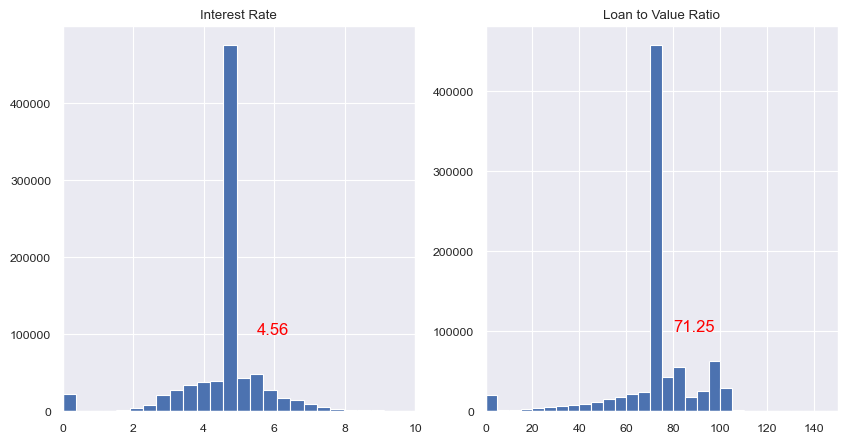
\includegraphics[width=0.85\textwidth]{CHXX_Numerical_Distributions_2.png}
    \caption*{The results of the KNNImputer applying mean (annotated in red) values for all missing values show clearly here by the high amount of values at the mean.}
    \label{fig:CHXX_Numerical_Distributions_2}
\end{figure}

% Add analysis of categorical features

% Correlation Analysis?

\subsection{Fairness}\label{subsec:Fairness}

% Probably rename - tie to Hypothesis and Research Questions

Potential unfairness in the underlying data can be identified from assessing the distribution of the target variable across different groups.
\textbf{Figure \ref{fig:CHXX_Loan_Grant_By_Protected_Attribute}} shows the amount of (not) granted loans per race and by sex, the probabilities of being granted a loan across these groups can be found in \textbf{Table \ref{tab:loan_granting}}.\@

\begin{figure}[h]
    \centering
    \caption{Loan Grant by Protected Attribute}
    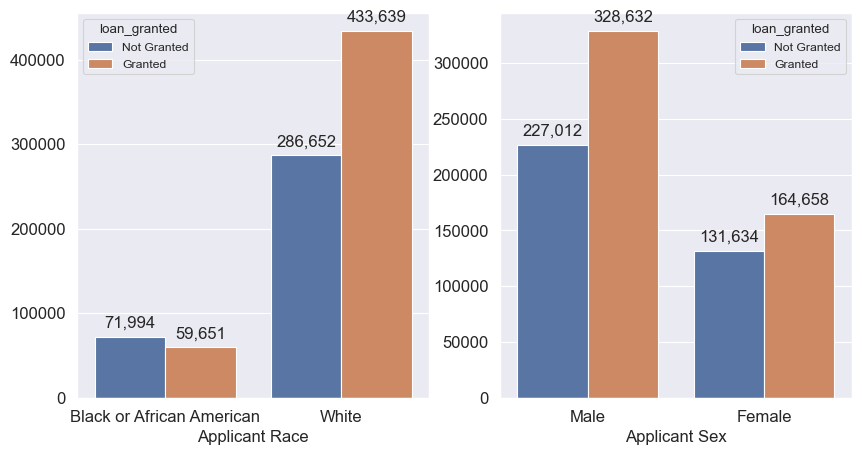
\includegraphics[width=0.85\textwidth]{CHXX_Loan_Grant_By_Protected_Attribute.png}
    \caption*{Discrimination by race is apparent in the data, as the amount of granted loans differs significantly}
    \label{fig:CHXX_Loan_Grant_By_Protected_Attribute}
\end{figure}

\begin{table}[htbp]
    \centering
      \caption{Loan Granting Statistics by Applicant Race and Sex}
      \begin{tabular}{lcc}
      \toprule
      \textbf{Applicant Race} & \textbf{Applicant Sex} & \textbf{Loan Granted (\%)} \\
      \midrule
      Black or African American & Male    & 46.4 \\
            & Female  & 44.1 \\
      White & Male    & 60.9 \\
            & Female  & 58.8 \\
      \bottomrule
      \end{tabular}
      \caption*{Regardless of their gender, Black or African American applicants are less likely to be granted a loan than White applicants.}
    \label{tab:loan_granting}%
\end{table}%

Even though the focus of the analysis is on the \textit{applicant\_race-1} attribute, \textit{applicant\_sex} has been included as a second discriminating factor, as it also constitutes a protected attribute.
Inspection of the results depicted here did however imply that the issue of racial equality is more pronounced than that of inequality between the sexes.
A chi-squared test of independence proved that assumption of underlying inequality between races in the data, as the p-value is \textit{<0.01} and therefore H0 (equality in granted loans) could be rejected at any significance level.
Utilizing the aforementioned \textbf{AIF360} package to assess the mean difference of granted loans between the races in the underlying data amounted to a \textit{14.9\%} difference.

\subsection{Enrichment Data}\label{subsec:Enrichment_Data}

% Describe and put all important graphs in here and leave fairness assessment for discussion 

\textbf{Figure \ref{fig:Scatter_White_Applicants_Loan_Grant}} shows a scatterplot that relates the percentage of white applicants to the percentage of granted loans per county. It indicates that a higher percentage of white applicants per county does not only seem to be correlated with a higher percentage of these loans actually being granted, but also with a lower poverty rate on average.

\begin{figure}[h]
    \centering
    \caption{Relationship between Applicant Race, Poverty Rate and Loan Grants}
    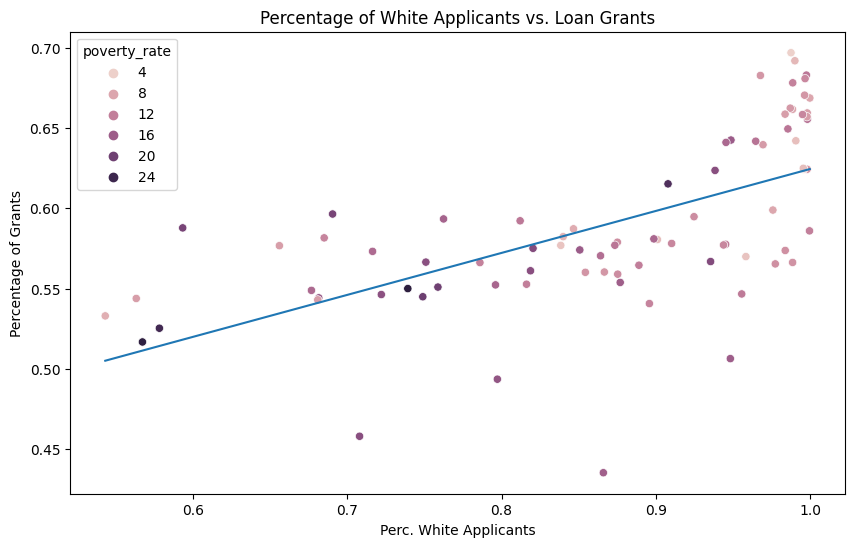
\includegraphics[width=0.85\textwidth]{images/CHXX_Perc_Grants_vs_Perc_White.png}
    \caption*{Counties with predominantly White applicants do not only tend to have a lower poverty rate on average, but also see a higher percentage of loans being granted on average.}
    \label{fig:Scatter_White_Applicants_Loan_Grant}
\end{figure}

It should however be noted that the distributions within the enrichment data themselves are skewed by nature, as there are way higher numbers of white applicants in the data set and only few counties have a substantial number of predicted mortgage grants (see \textbf{Figure \ref{fig:Enrichment_Data_EDA}}).

\begin{figure}[h]
    \centering
    \caption{Enrichment Data EDA}
    \begin{minipage}{0.33\textwidth}
        \centering
        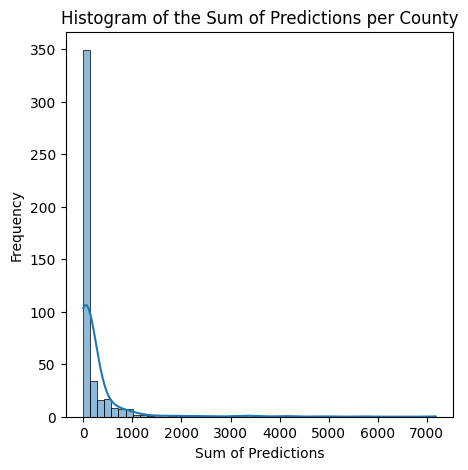
\includegraphics[width=\textwidth]{images/geo_enrich/predictions_per_county.png}
    \end{minipage}\hfill
    \begin{minipage}{0.33\textwidth}
        \centering
        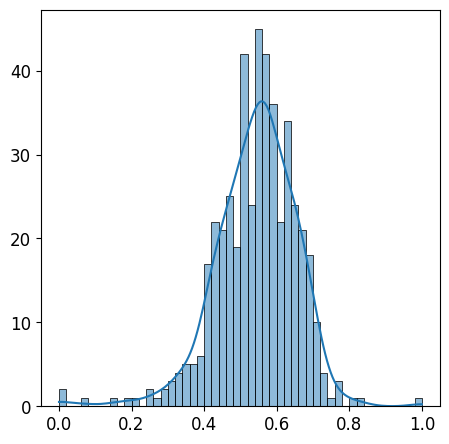
\includegraphics[width=\textwidth]{images/geo_enrich/perc_predictions.png}
    \end{minipage}\hfill
    \begin{minipage}{0.33\textwidth}
        \centering
        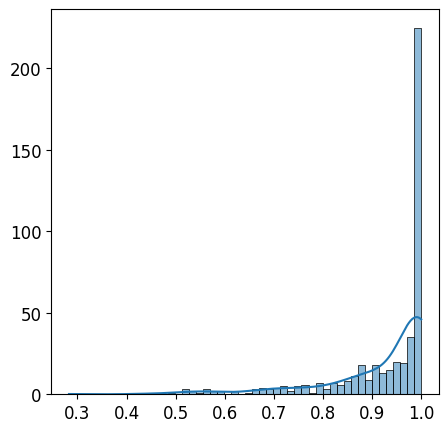
\includegraphics[width=\textwidth]{images/geo_enrich/white_per_county.png}
    \end{minipage}\hfill
    \label{fig:Enrichment_Data_EDA}
    \caption*{Analyzing the enrichment data shows that while the percentage of predictions per county appears to be normally distributed, the distributions of the percentage of White applicants and the percentage of predicted granted loans per county are skewed.}
\end{figure}


\section{Results}\label{sec:Results}        

As defined in \textbf{Chapter \ref{subsec:Performance_Assessment}} and \textbf{Chapter \ref{subsec:Fairness_Assessment}}, the model is evaluated based on XXX



\subsection{Initial Performance}\label{subsec:Initial_Performance}

The initial run serving as a benchmark was conducted training the neural network described in \textbf{Chapter \ref{subsec:Model_Training_and_Prediction}} on the unadjusted training data (see \textbf{Chapter \ref{subsec:HMDA_Data}}).

\textbf{Explainability}

As was intended in \textbf{chapter \ref{subsec:Explainability}}, three different explainability algorithms were utilized to challenge each other's results and analyze overall patterns. \textbf{Figure \ref{fig:SHAP_explanations}} and \textbf{Figure \ref{fig:LIME_explanations}} show the individual explanations for the first 150 observations of the test set provided by SHAP and LIME, respectively. 
As already mentioned in \textbf{Chapter \ref{subsec:Performance_Assessment}}, the model behaved somewhat different from the expectations: Imputation of missing values in the \textit{debt\_to\_income\_ratio} feature led to a significant decrease in both fairness and performance measures of the model.
Therefore, it must be assumed that missingness in itself is not completely at random and holds information (or that the imputation method via a random forest regressor is not suitable for this task).
While SHAP considers that missingness to be the most important influence on model predictions, LIME weighs the \textit{debt\_to\_income\_ratio} features higher in general.
None of the algorithms consider the protected attributes to be of high direct impact on the results.

\begin{figure}[h]
    \centering
    \begin{minipage}{0.5\textwidth}
        \centering
        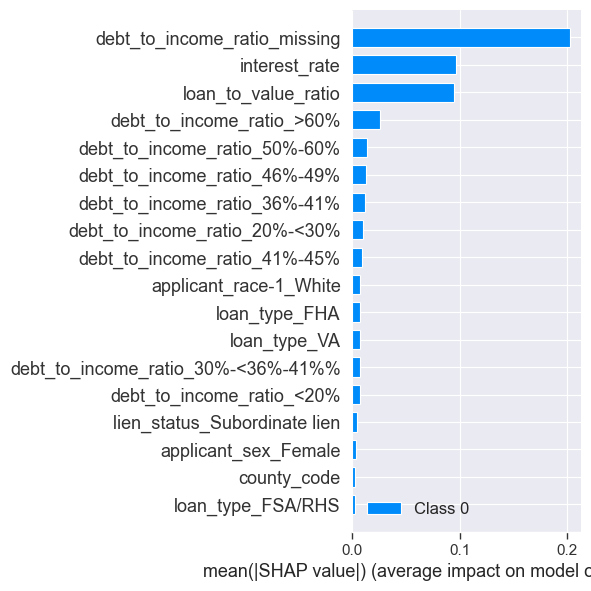
\includegraphics[width=\textwidth,height=5cm,keepaspectratio]{images/CHXX_UPDATE_SHAP_individual.png}
        \caption{SHAP individual explanations}
        \label{fig:SHAP_explanations}
    \end{minipage}\hfill
    \begin{minipage}{0.5\textwidth}
        \centering
        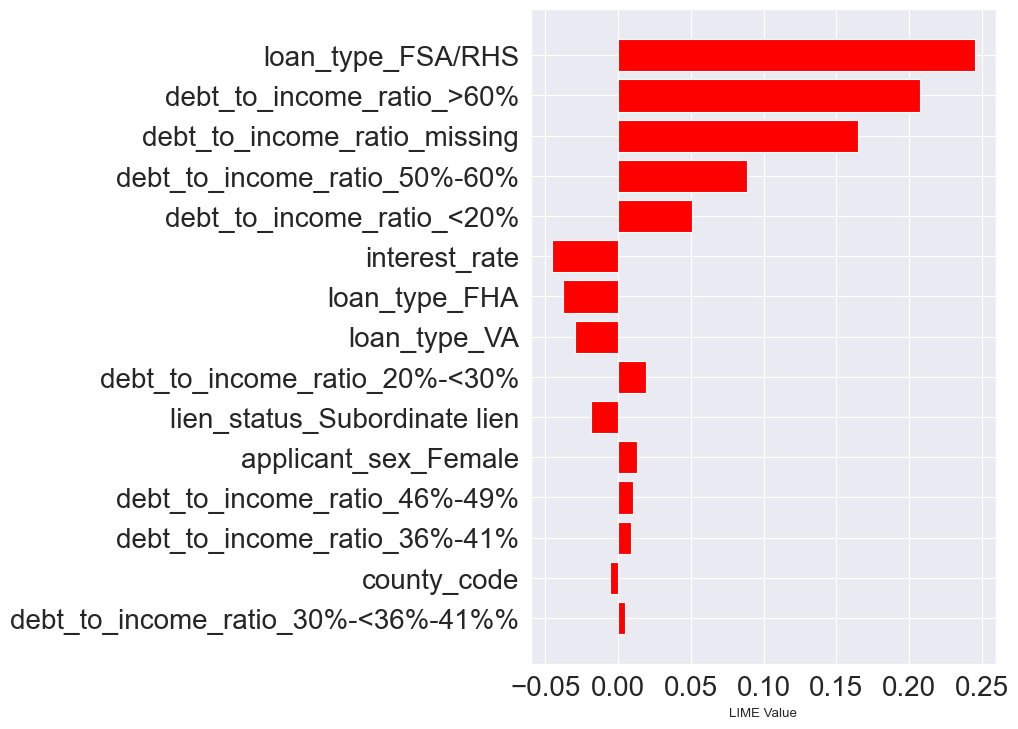
\includegraphics[width=\textwidth,height=5cm,keepaspectratio]{images/CHXX_UPDATE_LIME_individual.png}
        \caption{LIME individual explanations}
        \label{fig:LIME_explanations}
    \end{minipage}
    \caption*{Directly comparing LIME and SHAP explanations for the first 150 observations of the test set: While \textit{debt\_to\_income\_ratio} is an important factor in both explanations, its actual impact varies, as LIME also considers the \textit{loan\_type} feature to be of high importance. Default plotting options were kept: SHAP values are displayed as absolutes, while LIME values show the direction of their impact.}
\end{figure}

While the overall trends are similar with both algorithms, the actual impact of the features varies significantly. While this is not a direct threat to the quality of the results of this thesis, it is a reminder that explainability algorithms need to be analyzed carefully. 
This ties with the findings of Krishna et al. \parencite{Krishna2022}, who emphasize the importance of understanding the underlying assumptions of explainability algorithms and the need for a more comprehensive evaluation of their results.

To validate the results of the local explanations, a \textit{Global Surrogate Model} was used. \textbf{Figure \ref{fig:Global_Surrogate}} shows the results of the global surrogate model. Specifically, the five most important features according to the global surrogate model are compared to the SHAP and LIME explanations in terms of their relative performance.
It is apparent that the overall trends of SHAP and LIME are close to the global explanations.

\begin{figure}[h]
    \centering
    \caption{Global Surrogate Model compared to SHAP and LIME}
    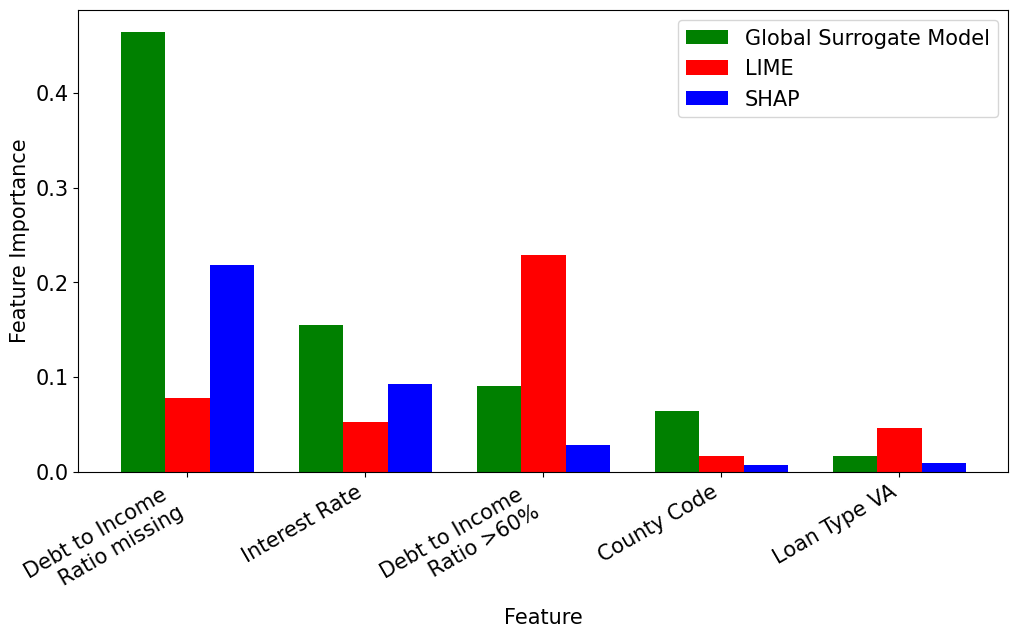
\includegraphics[width=0.85\textwidth]{images/CHXX_UPDATE_Surrogate_SHAP_LIME_combined.png}
    \caption*{Analyzing the 5 most important features according to the global surrogate model implies that the overall trends of SHAP and LIME are close to the global explanations.}
    \label{fig:Global_Surrogate}
\end{figure}

\textbf{Performance}

% Add performance results here (all iterations)

\textbf{Fairness}

% Add fairness results here (all iterations)

Table XXX shows the results of the initial model run as described in \textbf{Chapter \ref{sec:Methodology}}.

XXX Hier Tabelle von finalem Durchlauf XXX

XXX Basic Kommentare XXX

\subsection{Iteration I:\ Reweighing}\label{subsec:Iteration_I}

The results of the \textit{reweighed} model (see \textbf{Chapter \ref{subsec:Iterations}}) are promising. XXX

\subsection{Iteration II:\ Correlation Remover}\label{subsec:Iteration_II}

XXX

% Alle Ergebnisse einzeln oder am Ende Gesamttabelle mit allen Iterationen?

% \section{Limitations}\label{sec:Limitations} - hier oder am Ende?